\documentclass[conference]{IEEEtran}
\IEEEoverridecommandlockouts

\usepackage{cite}
\usepackage{amsmath,amssymb,amsfonts}
\usepackage{algorithm}
\usepackage[noend]{algpseudocode}
\usepackage{graphicx}
\usepackage{textcomp}
\usepackage{xcolor}
\usepackage{booktabs}
\usepackage{tikz}
\usetikzlibrary{arrows.meta,calc}
\usepackage{url}
\usepackage[hidelinks]{hyperref}

\newcommand{\code}[1]{\texttt{#1}}

% Model results are read from results.tex, which fill_results.py writes from
% gp_runs/results/runs.jsonl. A value that has not been measured prints as a bold "?".
\newcommand{\res}[1]{\ifcsname gp@#1\endcsname\csname gp@#1\endcsname\else\textbf{?}\fi}
\IfFileExists{results.tex}{\input{results.tex}}{}

\begin{document}

\title{GraphPatch: Graph-Verified Multi-Agent Repair of\\
Java Vulnerabilities with Open-Weight LLMs}

\author{
\IEEEauthorblockN{M. Sarmila}
\IEEEauthorblockA{\textit{Dept. of Artificial Intelligence and Data Science}\\
\textit{Dr. N.G.P. Institute of Technology}\\
Coimbatore, Tamil Nadu, India\\
sarmilamaruthachalam@gmail.com}
\and
\IEEEauthorblockN{Srikanth M}
\IEEEauthorblockA{\textit{Dept. of Artificial Intelligence and Data Science}\\
\textit{Dr. N.G.P. Institute of Technology}\\
Coimbatore, Tamil Nadu, India\\
23ad110@drngpit.ac.in}
\and
\IEEEauthorblockN{Tharshana S}
\IEEEauthorblockA{\textit{Dept. of Artificial Intelligence and Data Science}\\
\textit{Dr. N.G.P. Institute of Technology}\\
Coimbatore, Tamil Nadu, India\\
23ad117@drngpit.ac.in}
\and
\IEEEauthorblockN{Subhashini J}
\IEEEauthorblockA{\textit{Dept. of Artificial Intelligence and Data Science}\\
\textit{Dr. N.G.P. Institute of Technology}\\
Coimbatore, Tamil Nadu, India\\
24ltaid00001@drngpit.ac.in}
}

\maketitle

\begin{abstract}
LLM agents can now write patches for security vulnerabilities, and most repair systems
accept a patch once the code builds and the existing tests pass. Project tests rarely
contain an attack, so a patch can pass every test while untrusted input still reaches
the dangerous call. We present GraphPatch, a multi-agent repair framework for Java in
which one source-to-sink taint graph does two jobs: it selects the code the agents see,
and it decides, after the build and the tests, whether a candidate patch actually closed
the vulnerable path. A Planner, a Coder and a Critic work in a loop; when a candidate
still leaves a path open, the Critic receives that concrete path. Final verdicts use
held-out oracles that no agent sees: the paths removed by the developers' own fix, and
proof-of-vulnerability tests where they exist. The whole system runs on free and
open-source software, with the open-weight Qwen2.5-Coder-7B model served locally by
Ollama on a CPU-only laptop. On the taint checker's calibration over 115 CWE-Bench-Java
vulnerabilities, the developers' fix removes at least one reported path in 15 cases. On
the 9 of those that build and test in our environment, \res{all@stillvuln} of
\res{all@passing} LLM patches that passed the existing tests were still vulnerable.
GraphPatch verified
\res{full@V} of 9, against \res{single@V} for the single prompt, \res{nograph@V} for the
multi-agent baseline and 5 for a deterministic rule with no LLM.
\end{abstract}

\begin{IEEEkeywords}
automated vulnerability repair, taint analysis, program graphs, large language models,
open-weight models, multi-agent systems, patch validation
\end{IEEEkeywords}

\section{Introduction}

In December 2021, Log4Shell (CVE-2021-44228) showed how one data flow can put a large
part of the software ecosystem at risk. Attacker input reached a logging call inside a
widely used library, and thousands of projects were vulnerable without writing a single
line of unsafe code themselves. Many first-party vulnerabilities have the same shape.
Path traversal (CWE-22), OS command injection (CWE-78), cross-site scripting (CWE-79) and
code injection (CWE-94) all happen when untrusted data reaches a sensitive operation
without proper sanitization. A correct repair has to break that path.

LLM-based repair has moved fast. LLMs were first used directly for program
repair~\cite{xia2023apr} and for zero-shot vulnerability repair~\cite{pearce2023zeroshot};
they have since been fine-tuned for repair~\cite{huang2025finetune}, evaluated on
vulnerability tasks~\cite{yin2024multitask}, and turned into agents that browse a
repository, edit code and run tests~\cite{bouzenia2025repairagent}. Two limits remain.
First, most systems accept a patch once it compiles and the tests pass, and tests rarely
contain an attack, so a patch that does nothing about the vulnerability still looks
``plausible''. Second, many systems depend on large hosted models behind paid APIs,
which makes them hard to reproduce for students, small teams and researchers without a
budget, and sends the code under repair to a third party.

GraphPatch addresses both. Our contributions are:
\begin{itemize}
\item \textbf{One taint graph as context and as gate.} The same source-to-sink query
selects the methods the agents see and, re-run after every candidate, rejects patches
that build and pass the tests but leave the path open (Section~\ref{sec:approach}).
\item \textbf{Path-level feedback.} When the security gate fails, the Critic receives
the surviving path with file and line, not only a pass/fail signal.
\item \textbf{A held-out evaluation protocol.} The final verdict uses the paths removed
by the developers' fix and proof-of-vulnerability tests, which no agent sees, and the
checker itself is calibrated against the developers' fixes before any repair
(Section~\ref{sec:setup}).
\item \textbf{A fully free and open-source stack.} An open-weight 7B code model served
locally on a laptop CPU, open parsers, build tools and public benchmarks; no step needs
a paid API, a commercial licence or a GPU (Table~\ref{tab:stack}).
\end{itemize}

\section{Related Work}

\subsection{LLM-Based Program and Vulnerability Repair}
Huang et al.~\cite{huang2025finetune} study how fine-tuning code LLMs affects automated
program repair, and Yin et al.~\cite{yin2024multitask} evaluate open-source LLMs on
vulnerability detection, assessment, localization and description. Xia et
al.~\cite{xia2023apr} showed that LLMs applied directly to repair outperform earlier
learning-based tools, and Yang et al.~\cite{yang2025unnatural} rank candidate patches
with LLM entropy. For security, Pearce et al.~\cite{pearce2023zeroshot} found that LLMs
repair simple vulnerabilities zero-shot but struggle with real ones; Zhang et
al.~\cite{zhang2024pretrained} study pre-trained models for vulnerability repair,
LLM4CVE~\cite{fakih2025llm4cve} repairs real-world vulnerabilities with an iterative
pipeline, and Zhao et al.~\cite{zhao2025secure} study the security of LLM-generated code
across CWE types. Closest to our work, LoopRepair~\cite{ye2026looprepair} iteratively
repairs C/C++ vulnerabilities and uses taint statement coverage to choose which
test-failing candidate to refine. GraphPatch instead uses a static source-to-sink path as
an acceptance gate after the tests pass, and judges final patches with security checks
the loop never sees.

\subsection{Agentic and Multi-Agent Software Engineering}
RepairAgent~\cite{bouzenia2025repairagent} lets an LLM agent call tools to read code,
edit it and run tests, and repairs real bugs from Defects4J. Its acceptance criterion
remains functional. Because test-passing patches can still be wrong, patch correctness
assessment has become its own problem~\cite{zhou2024patchcorrect}. GraphPatch keeps the
separation of roles but adds a security-specific gate and gives its Critic the concrete
surviving path.

\subsection{Program Graphs and Static Analysis with LLMs}
Code property graphs~\cite{yamaguchi2014cpg} merge syntax, control flow and data flow
into one graph for vulnerability discovery, and the open-source tool Joern~\cite{joern}
implements them at scale. ROCODE~\cite{jiang2025rocode} integrates program analysis into
LLM code generation and backtracks when the analysis finds an error. Fine-tuned LLMs
have been applied to vulnerability detection~\cite{shestov2025finetune}, but Ding et
al.~\cite{ding2025vulndetect} show that code models still perform poorly on realistic
benchmarks. IRIS~\cite{li2025iris} combines LLM-inferred source and sink specifications
with static taint analysis and introduced CWE-Bench-Java. GraphPatch uses a much lighter
graph, so it can be rebuilt after every candidate in about a second on a laptop.

\section{Approach}
\label{sec:approach}

\begin{figure*}[t]
\centering
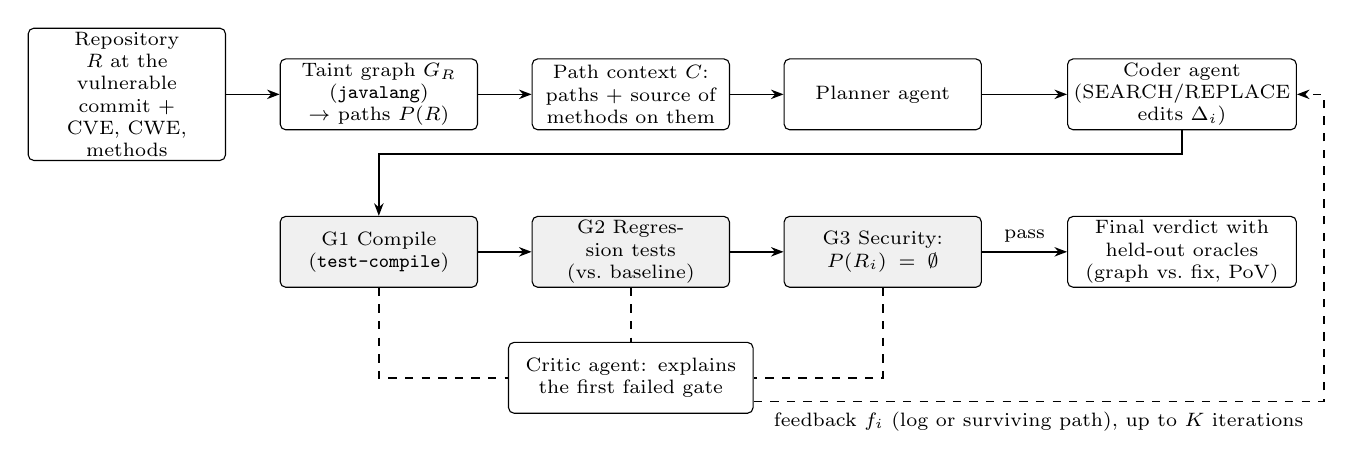
\begin{tikzpicture}[
  x=1mm, y=1mm, font=\scriptsize,
  box/.style={draw, rounded corners=2pt, align=center, minimum height=9mm,
              inner sep=1.5pt, text width=#1},
  box/.default=24mm,
  gate/.style={box=#1, fill=gray!12},
  gate/.default=24mm,
  arr/.style={-{Stealth[length=1.6mm]}, semithick}]
  \node[box] (in)    at (14,0)    {Repository $R$ at the\\vulnerable commit +\\CVE, CWE, methods};
  \node[box] (tg)    at (46,0)    {Taint graph $G_R$\\(\code{javalang})\\$\rightarrow$ paths $P(R)$};
  \node[box] (ctx)   at (78,0)    {Path context $C$:\\paths + source of\\methods on them};
  \node[box] (plan)  at (110,0)   {Planner agent};
  \node[box=28mm] (coder) at (148,0) {Coder agent\\(SEARCH/REPLACE\\edits $\Delta_i$)};
  \node[gate] (g1) at (46,-20)  {G1 Compile\\(\code{test-compile})};
  \node[gate] (g2) at (78,-20)  {G2 Regression tests\\(vs.\ baseline)};
  \node[gate] (g3) at (110,-20) {G3 Security:\\$P(R_i)=\emptyset$};
  \node[box=28mm] (out) at (148,-20) {Final verdict with\\held-out oracles\\(graph vs.\ fix, PoV)};
  \node[box=30mm] (critic) at (78,-36) {Critic agent: explains\\the first failed gate};

  \draw[arr] (in) -- (tg);
  \draw[arr] (tg) -- (ctx);
  \draw[arr] (ctx) -- (plan);
  \draw[arr] (plan) -- (coder);
  \draw[arr] (coder.south) -- ++(0,-3) -| (g1.north);
  \draw[arr] (g1) -- (g2);
  \draw[arr] (g2) -- (g3);
  \draw[arr] (g3) -- node[above]{pass} (out);
  \draw[dashed, semithick] (g1.south) |- (critic.west);
  \draw[dashed, semithick] (g2.south) -- (critic.north);
  \draw[dashed, semithick] (g3.south) |- (critic.east);
  \draw[arr, dashed] (critic.east) ++(0,-3) -- (166,-39)
     node[pos=0.5, below]{feedback $f_i$ (log or surviving path), up to $K$ iterations}
     -- (166,0) -- (coder.east);
\end{tikzpicture}
\caption{Overview of GraphPatch. The taint graph gives the agents their context and,
re-built on every candidate, acts as the security gate G3. Each candidate passes three
gates in order of cost; the first failure is explained by the Critic and fed back to
the Coder, up to $K$ iterations. Held-out oracles used for the final verdict
(Section~\ref{sec:oracles}) are not shown to any agent.}
\label{fig:overview}
\end{figure*}

Fig.~\ref{fig:overview} gives an overview. The input is a repository $R$ checked out at
a vulnerable commit, the CVE and its CWE class, and the methods the benchmark marks as
vulnerable. The output is either a patch $\Delta$ that passed every gate, or the last
candidate after $K$ iterations, together with the evidence for the verdict.

\subsection{Problem Definition}
Let $G_R=(V,E)$ be the taint graph of $R$. For a CWE class $c$, a specification
$S_c=(\mathit{Src}_c, \mathit{Snk}_c, \mathit{San}_c)$ lists sources (parameters of the
vulnerable methods, HTTP request getters, archive entry names), sinks (e.g.,
\code{new File} or \code{FileOutputStream} for CWE-22, \code{Runtime.exec} for CWE-78,
\code{out.print} for CWE-79, expression parsers for CWE-94) and recognized sanitizers and
guards (e.g., path canonicalization followed by a containment check). The set of
vulnerable paths is
\begin{equation}
P(R)=\{\,p\in \mathit{Flows}(G_R,\mathit{Src}_c,\mathit{Snk}_c) \mid
p\cap \mathit{San}_c=\emptyset\,\},
\label{eq:paths}
\end{equation}
where $\mathit{Flows}$ is the set of data-flow paths in $G_R$ from a source to a sink
and $p\cap \mathit{San}_c=\emptyset$ means that $p$ passes through no recognized
sanitizer or guard. A candidate patch $\Delta$ is applied as $R' = R \oplus \Delta$ on a
clean copy of $R$. Inside the loop, $R'$ passes if it compiles, keeps every test of $R$
that passed before, and $P(R')=\emptyset$. Because the analysis is approximate, passing
the gates is not our definition of a correct fix; the final verdict uses held-out
oracles (Section~\ref{sec:oracles}).

\subsection{Taint Graph}
\label{sec:graph}
Each Java file is parsed with the open-source \code{javalang} parser. The graph has three
kinds of edges: data flow inside a method (assignments, declarations, call arguments);
field flow inside a class (a tainted field is tainted in every method of the class);
and call edges between analysed methods (a tainted argument taints the callee's
parameter, and a tainted return value taints the call result). The analysed files are
the vulnerable files and up to 60 files of the same package. A guard such as
\code{if (!f.getCanonicalPath().startsWith(base)) throw \ldots} cleans the variables it
checks from that line on. Sources, sinks and sanitizers come from per-CWE catalogues.
The analysis is flow-insensitive within a method and is an approximation, not a sound
analysis; Section~\ref{sec:calib} measures how often it agrees with the developers'
fixes.

\subsection{Path-Sliced Context}
The context $C$ given to the agents contains every path in $P(R)$ as an ordered list of
statements with file and line, followed by the numbered source of each method on those
paths (at most 12 methods). Compared with whole vulnerable files, this context is
shorter and points the model at the statements that matter, which is especially
important for a small local model whose context window and memory are limited.

\subsection{Agents and Repair Loop}
\label{sec:loop}
Three LLM agents and one deterministic validator take part; all agents use the same
model.
\begin{itemize}
\item \textbf{Planner} reads the CWE description, the paths and $C$, and states where
each path should be broken (validate at the source, sanitize before the sink, or replace
the sink with a safe API).
\item \textbf{Coder} writes the change as SEARCH/REPLACE edits on the real files. An
edit whose SEARCH text does not occur exactly once is reported back as a failure.
\item \textbf{Critic} is called only after a gate fails. It receives the diff and the
compiler log, the failing tests, or the surviving paths in $P(R_i)$, and returns a short
explanation of what to change.
\item \textbf{Validator} is not an LLM. It applies the edits to a clean checkout and runs
the gates with Maven or Gradle, either in Docker or with local JDKs.
\end{itemize}
Algorithm~\ref{alg:loop} shows the loop. G1 compiles the main and test sources. G2 runs
the tests of the affected module and compares them with a baseline run on the unpatched
commit, so pre-existing failures are not counted against a patch. G3 rebuilds the taint
graph of $R_i$ and re-runs the query of Eq.~(\ref{eq:paths}). The first failure goes to
the Critic. If the budget runs out, the last candidate $\Delta_K$ is judged by the
held-out oracles like any other; we do not fall back to an earlier candidate.

\begin{algorithm}[t]
\caption{Graph-verified repair loop}
\label{alg:loop}
\small
\begin{algorithmic}[1]
\Require repository $R$, CVE $a$, specification $S_c$, budget $K$
\State $P_0 \gets \Call{Paths}{\textsc{TaintGraph}(R), S_c}$
\State $T_0 \gets$ tests passing on $R$; $f \gets \emptyset$
\State $C \gets \Call{PathContext}{R, P_0}$; $\pi \gets \Call{Planner}{a, P_0, C}$
\For{$i = 1$ \textbf{to} $K$}
  \State $\Delta_i \gets \Call{Coder}{\pi, C, f}$; $R_i \gets R \oplus \Delta_i$
  \For{$g \in \langle \textsc{Compile}, \textsc{Tests}_{T_0}, \textsc{Security}_{S_c}\rangle$}
    \If{\textbf{not} $g(R_i)$}
      \State $f \gets \Call{Critic}{\Delta_i, \textsc{Evidence}(g)}$
      \State \textbf{continue} outer loop
    \EndIf
  \EndFor
  \State \Return $\Delta_i$ \Comment{passes all gates}
\EndFor
\State \Return $\Delta_K$ \Comment{unresolved in-loop}
\end{algorithmic}
\end{algorithm}

\subsection{Developer Tooling}
The same analysis is packaged for everyday use, without any model or key: a SARIF~2.1.0
export~\cite{sarif} that any SARIF-compatible viewer or CI system can display; a git
pre-commit hook that blocks a commit when a staged Java file has a taint path; a
generator of JUnit attack tests that try to write outside the target folder for each
path-traversal finding; a check of declared Maven and Gradle dependencies against the
free OSV database~\cite{osv}; and a FastAPI web interface that shows each path as a
source-to-sink graph next to the code, runs the repair loop, and replays saved benchmark
runs.

\section{Experimental Setup}
\label{sec:setup}

\subsection{Research Questions}
\begin{itemize}
\item \textbf{RQ1 (Test-passing but vulnerable):} How many patches that compile and pass
all existing tests still fail a held-out security oracle?
\item \textbf{RQ2 (Effectiveness):} How many vulnerabilities does GraphPatch fix with a
verified patch, compared with a rule, a single prompt and a multi-agent baseline without
the graph?
\item \textbf{RQ3 (Ablation):} What do the path-sliced context and the security gate
each contribute?
\item \textbf{RQ4 (Cost):} How large is the context, and how many iterations, tokens and
seconds does each system need on a CPU-only laptop?
\end{itemize}

\subsection{Benchmark}
CWE-Bench-Java~\cite{li2025iris} contains 120 vulnerabilities from real Java projects
(CWE-22, 78, 79, 94) with the vulnerable and fixed versions; 115 have their vulnerable
code in main sources. As in most repair studies, we assume perfect fault localization:
the vulnerable methods named by the benchmark are given, and their parameters are also
used as taint sources.

\begin{table}[t]
\centering
\caption{Calibration of the taint query on the 115 CWE-Bench-Java vulnerabilities with
main-source fixes}
\label{tab:calib}
\begin{tabular}{lrrrr}
\toprule
CWE & CVEs & Path & Fix removes & Fix removes \\
    &      & found & all & $\ge$1 \\
\midrule
CWE-22 & 53 & 21 & 8 & 13 \\
CWE-78 & 13 & 1 & 1 & 1 \\
CWE-79 & 29 & 8 & 0 & 1 \\
CWE-94 & 20 & 3 & 0 & 0 \\
\midrule
All & 115 & 33 & 9 & 15 \\
\bottomrule
\end{tabular}
\end{table}

\subsection{Calibration of the Security Gate}
\label{sec:calib}
Before any repair we ran the taint query on the vulnerable and the fixed version of every
vulnerability (Table~\ref{tab:calib}). The query reports at least one path on the
vulnerable version for 33 of 115; the developers' fix removes all reported paths in 9
cases and at least one in 15. Many CWE-79 vulnerabilities in the benchmark are bugs
inside HTML sanitizer libraries, and many CWE-94 fixes change evaluation contexts; a
source-to-sink check cannot express such fixes. We also ran the calibration on the 65
Vul4J~\cite{bui2022vul4j} vulnerabilities whose developer fix builds and passes its
proof-of-vulnerability tests in our harness: the fix removes a reported path in only 4,
because most weakness types there (input validation, infinite loops, XXE) are outside
the catalogues. We therefore evaluate repair on the 15 CWE-Bench-Java vulnerabilities
whose fix removes at least one path, the only ones the graph oracle can judge. Six of
them do not build or test in our environment and are excluded, which leaves 9, all
CWE-22.

Two harness checks guard against a broken pipeline. With no change applied, none of the
6 CVEs we tested is verified; with the developers' fix applied, 5 of 6 are verified. The
sixth (Spark, CVE-2018-9159) cannot be judged: its fix removes none of the reported
paths and it has no proof-of-vulnerability test.

\subsection{Held-Out Oracles and Verdicts}
\label{sec:oracles}
The final verdict uses oracles that no agent sees. \emph{Graph-versus-fix:} the patch
must remove every path that the developers' fix removes. In the loop the agents are
asked to remove every reported path, since nothing else is known at repair time; the
verdict only requires the paths the real fix removes, because the calibration shows that
real fixes often leave some reports in place. \emph{PoV tests:} tests added or changed
by the fix commit that fail on the vulnerable version and pass on the developers' fix,
used where they exist. A patch is \emph{Verified} if it compiles, causes no new test
failures and passes every oracle that applies; \emph{Plausible} if it compiles and causes
no new test failures but fails an oracle; and \emph{Rejected} otherwise.

\subsection{Compared Systems}
All LLM-based systems use the same model, the same validator and, where they loop, an
iteration budget of $K=3$.
\begin{itemize}
\item \textbf{B0 Rule (no LLM):} for each path-traversal path, a fixed rule normalizes
the tainted path and checks that it stays inside the base directory.
\item \textbf{B1 Single prompt:} one LLM call with the vulnerable files and the CWE
description, no feedback.
\item \textbf{B3 Multi-agent, tests only:} Planner, Coder and Critic with whole files as
context and only gates G1 and G2.
\item \textbf{GraphPatch:} path-sliced context and all three gates.
\item \textbf{Ablations (RQ3):} $-$context (whole files, all three gates) and $-$G3
(path-sliced context, no security gate).
\end{itemize}

\subsection{Model and Implementation}
\label{sec:impl}
All agents use Qwen2.5-Coder-7B-Instruct~\cite{hui2024qwen25coder}, an open-weight code
model released under the Apache~2.0 licence, served locally with Ollama~\cite{ollama}
through its OpenAI-compatible endpoint at temperature~0. Ollama's default context window
of 2,048 tokens silently truncates our prompts, so we raise it to 24,576 tokens, and the
harness stops a run when the prompt token count reported by the server is far below the
prompt length. Replies are limited to 4,096 tokens. GraphPatch is implemented in Python;
Table~\ref{tab:stack} lists every component. Builds and tests run with Maven or Gradle on
Eclipse Temurin JDK 8 or 17. Experiments ran on a laptop with an AMD Ryzen~5~5625U and
16\,GB of RAM, CPU only, without a GPU. No step requires a paid API, a commercial
licence or a cloud service. Each configuration is run once per vulnerability at
temperature~0. Source code, prompts and all run artifacts (every prompt, reply, diff and
verdict) will be made publicly available upon publication.

\begin{table}[t]
\centering
\caption{Software used by GraphPatch and its evaluation. Every component is free of
charge and open-source.}
\label{tab:stack}
\footnotesize
\setlength{\tabcolsep}{3pt}
\begin{tabular}{lll}
\toprule
Role & Component & Licence \\
\midrule
LLM (all agents) & Qwen2.5-Coder-7B-Instruct & Apache-2.0 \\
LLM serving & Ollama & MIT \\
Java parsing, taint graph & javalang & MIT \\
Implementation & Python, FastAPI, Uvicorn & PSF, MIT, BSD-3 \\
Build, test & Maven, Gradle, JUnit & Apache-2.0, EPL \\
JDK & Eclipse Temurin 8/17 & GPLv2 + CE \\
Isolation (optional) & Docker Engine & Apache-2.0 \\
Unit tests & pytest & MIT \\
Report format & SARIF 2.1.0 (OASIS) & Open standard \\
Benchmarks & CWE-Bench-Java, Vul4J & public, CC-BY-4.0 \\
\bottomrule
\end{tabular}
\end{table}

\section{Results}
\label{sec:results}

\begin{table}[t]
\centering
\caption{Outcome per vulnerability on CWE-Bench-Java. V = verified, P = plausible but
fails a held-out oracle, R = rejected, E = run error; iterations in parentheses.}
\label{tab:java}
\begin{tabular}{lcccc}
\toprule
CVE (all CWE-22) & B0 & B1 & B3 & GraphPatch \\
\midrule
CVE-2022-25842   & V & \res{single@CVE-2022-25842} & \res{nograph@CVE-2022-25842} & \res{full@CVE-2022-25842} \\
CVE-2018-1002201 & P & \res{single@CVE-2018-1002201} & \res{nograph@CVE-2018-1002201} & \res{full@CVE-2018-1002201} \\
CVE-2018-1002200 & V & \res{single@CVE-2018-1002200} & \res{nograph@CVE-2018-1002200} & \res{full@CVE-2018-1002200} \\
CVE-2018-1002202 & V & \res{single@CVE-2018-1002202} & \res{nograph@CVE-2018-1002202} & \res{full@CVE-2018-1002202} \\
CVE-2018-17297   & P & \res{single@CVE-2018-17297} & \res{nograph@CVE-2018-17297} & \res{full@CVE-2018-17297} \\
CVE-2020-35460   & V & \res{single@CVE-2020-35460} & \res{nograph@CVE-2020-35460} & \res{full@CVE-2020-35460} \\
CVE-2018-12036   & V & \res{single@CVE-2018-12036} & \res{nograph@CVE-2018-12036} & \res{full@CVE-2018-12036} \\
CVE-2022-31194   & P & \res{single@CVE-2022-31194} & \res{nograph@CVE-2022-31194} & \res{full@CVE-2022-31194} \\
CVE-2022-26049   & R & \res{single@CVE-2022-26049} & \res{nograph@CVE-2022-26049} & \res{full@CVE-2022-26049} \\
\bottomrule
\end{tabular}
\end{table}

\begin{table}[t]
\centering
\caption{Summary over the 9 evaluated vulnerabilities (medians per vulnerability for
iterations, tokens and time)}
\label{tab:summary}
\begin{tabular}{lrrrr}
\toprule
 & B0 & B1 & B3 & GraphPatch \\
\midrule
Verified                     & 5 & \res{single@V} & \res{nograph@V} & \res{full@V} \\
Plausible (still vulnerable) & 3 & \res{single@P} & \res{nograph@P} & \res{full@P} \\
Rejected                     & 1 & \res{single@R} & \res{nograph@R} & \res{full@R} \\
Run errors                   & 0 & \res{single@E} & \res{nograph@E} & \res{full@E} \\
Iterations                   & 1 & 1 & \res{nograph@iters} & \res{full@iters} \\
Input tokens                 & 0 & \res{single@intok} & \res{nograph@intok} & \res{full@intok} \\
Output tokens                & 0 & \res{single@outtok} & \res{nograph@outtok} & \res{full@outtok} \\
Time (s)                     & 292 & \res{single@secs} & \res{nograph@secs} & \res{full@secs} \\
\bottomrule
\end{tabular}
\end{table}

\subsection{RQ1: Test-Passing Patches That Remain Vulnerable}
Across the three LLM-based systems, \res{single@passing}, \res{nograph@passing} and
\res{full@passing} final patches (B1, B3, GraphPatch) compiled and passed the existing
tests. Of these, \res{single@stillvuln}, \res{nograph@stillvuln} and
\res{full@stillvuln} still failed a held-out oracle (Table~\ref{tab:summary}, Plausible).
The rule baseline shows why the oracle is needed even without an LLM: on 3 of 9
vulnerabilities its containment checks compiled and passed every test but still
failed a held-out oracle. On CVE-2018-1002201 (zt-zip), for example, a second,
backslash-aware unpacking routine passes entry names to \code{FileUtils.forceMkdir} and
\code{FileUtils.copy}; a patch that guards only the main unpacking routine passes all
118 existing tests and is still vulnerable.

\subsection{RQ2: Effectiveness}
Table~\ref{tab:java} shows each system on each vulnerability. GraphPatch verified
\res{full@V} of 9, B1 \res{single@V}, B3 \res{nograph@V} and the rule B0 5.

\begin{table}[t]
\centering
\caption{Ablation on the 9 vulnerabilities}
\label{tab:ablation}
\begin{tabular}{lccc}
\toprule
Variant & Verified & Plausible & Rejected \\
\midrule
GraphPatch & \res{full@V} & \res{full@P} & \res{full@R} \\
$-$context (whole files) & \res{filectx@V} & \res{filectx@P} & \res{filectx@R} \\
$-$G3 (no security gate) & \res{nogate@V} & \res{nogate@P} & \res{nogate@R} \\
B3 (neither) & \res{nograph@V} & \res{nograph@P} & \res{nograph@R} \\
\bottomrule
\end{tabular}
\end{table}

\subsection{RQ3: Ablation}
Table~\ref{tab:ablation} removes one component at a time. Without the security gate,
\res{nogate@P} patches were accepted in the loop although they fail a held-out oracle,
against \res{full@P} with it. With whole files instead of the path-sliced context,
\res{filectx@V} vulnerabilities were verified, against \res{full@V}.

\subsection{RQ4: Context Size and Cost}
The path-sliced context had a median of 6,184 characters against 11,861 for the whole
vulnerable files, a median reduction of 48\% (32\% to 83\% per vulnerability). This
context is built before any model call, so the reduction does not depend on the model.
GraphPatch's median input was \res{full@intok} tokens per vulnerability, against
\res{nograph@intok} for B3 and \res{single@intok} for B1, and its median time was
\res{full@secs}\,s, against \res{nograph@secs}\,s and \res{single@secs}\,s, on the
CPU-only laptop. Because every component is free, we report cost as tokens and time
rather than money.

\section{Discussion}

\subsection{What a Rule Can Already Do}
B0 verified 5 of the 9 vulnerabilities without any LLM. Most path-traversal fixes in
this set use the same containment check, so a rule placed at the reported path is a
strong baseline. Its limits show on harder cases: many paths through several methods
(CVE-2018-17297, 16 paths), or a check that must fit the project's tests
(CVE-2022-26049, rejected). Seeding the Coder with the rule's patch as its first
candidate is a natural combination.

\subsection{Why the Security Gate Is Not Plain Reachability}
A tempting simplification is to accept a patch once the sink is no longer reachable
from the source in the call graph. This fails: a correct fix adds a guard on the
existing path and removes no call edge. The gate therefore uses a sanitizer-aware taint
query that treats a recognized guard as breaking the path.

\subsection{Threats to Validity}
\emph{Internal validity.} The security gate depends on a lightweight, flow-insensitive
analysis and on hand-written catalogues; guards are recognized by shape, so a patch could
add a check that looks right but checks nothing useful. The graph-versus-fix oracle uses
the same query as gate G3, which favors GraphPatch; proof-of-vulnerability tests are the
independent check where they exist. On Vul4J, the rule B0 removed every reported path on
VUL4J-41 and VUL4J-43 yet still failed the PoV tests, which shows that the graph oracle
can be optimistic. \emph{External validity.} The evaluated set is small (9) and all
CWE-22, the language is Java only, and we use one 7B model; results may differ for
other weakness types, languages and larger models. \emph{Data leakage.} Fixes in public
benchmarks may be in the model's training data. \emph{Non-determinism.} Each
configuration is run once at temperature~0; with 9 vulnerabilities we report counts per
vulnerability and make no significance claims.

\section{Conclusion and Future Work}
Passing the tests is not the same as fixing the vulnerability. GraphPatch uses one taint
graph to choose what the agents see and to check, after every candidate, that the
vulnerable path is closed, and it judges final patches with oracles the agents never
see. It runs entirely on free and open-source software with a 7B open-weight model on a
laptop CPU, so any group can reproduce and extend it without a budget. On 9 CWE-Bench-Java
vulnerabilities it verified \res{full@V}, against \res{single@V} for a single prompt and
\res{nograph@V} for a multi-agent baseline without the graph.

Future work follows from the threats above. A Tree-sitter~\cite{treesitter} front end
would let one graph serve several languages; a reachability-based slice could replace
the fixed method limit of the context; open-source analyses such as Joern~\cite{joern}
could cover more weakness types; dependency advisories from OSV~\cite{osv} could be
repaired by safe version upgrades checked by the same gates, including breaking
updates~\cite{reyes2024bump}; and a minimal-patch check before the build, together with
a per-attempt evidence database, would make repairs cheaper and easier to audit.

\begin{thebibliography}{00}
\bibitem{xia2023apr} C. S. Xia, Y. Wei, and L. Zhang, ``Automated program repair in the
era of large pre-trained language models,'' in \textit{Proc. IEEE/ACM 45th Int. Conf.
Software Engineering (ICSE)}, 2023, pp. 1482--1494, doi: 10.1109/ICSE48619.2023.00129.
\bibitem{pearce2023zeroshot} H. Pearce, B. Tan, B. Ahmad, R. Karri, and B. Dolan-Gavitt,
``Examining zero-shot vulnerability repair with large language models,'' in \textit{Proc.
IEEE Symp. Security and Privacy (SP)}, 2023, pp. 2339--2356, doi:
10.1109/SP46215.2023.10179324.
\bibitem{huang2025finetune} K. Huang, J. Zhang, X. Bao, X. Wang, and Y. Liu,
``Comprehensive fine-tuning large language models of code for automated program
repair,'' \textit{IEEE Trans. Software Engineering}, vol. 51, no. 4, pp. 904--928, Apr.
2025, doi: 10.1109/TSE.2025.3532759.
\bibitem{yin2024multitask} X. Yin, C. Ni, and S. Wang, ``Multitask-based evaluation of
open-source LLM on software vulnerability,'' \textit{IEEE Trans. Software Engineering},
2024, doi: 10.1109/TSE.2024.3470333.
\bibitem{bouzenia2025repairagent} I. Bouzenia, P. Devanbu, and M. Pradel, ``RepairAgent:
An autonomous, LLM-based agent for program repair,'' in \textit{Proc. IEEE/ACM 47th Int.
Conf. Software Engineering (ICSE)}, 2025, doi: 10.1109/ICSE55347.2025.00157.
\bibitem{jiang2025rocode} X. Jiang, Y. Dong, Y. Tao, H. Liu, Z. Jin, and G. Li, ``ROCODE:
Integrating backtracking mechanism and program analysis in large language models for code
generation,'' in \textit{Proc. IEEE/ACM 47th Int. Conf. Software Engineering (ICSE)},
2025, pp. 334--346, doi: 10.1109/ICSE55347.2025.00133.
\bibitem{yang2025unnatural} A. Z. H. Yang, S. Kolak, V. J. Hellendoorn, R. Martins, and
C. Le Goues, ``Revisiting unnaturalness for automated program repair in the era of large
language models,'' in \textit{Proc. IEEE/ACM 47th Int. Conf. Software Engineering
(ICSE)}, 2025, pp. 2561--2573, doi: 10.1109/ICSE55347.2025.00089.
\bibitem{zhang2024pretrained} Q. Zhang, C. Fang, B. Yu, W. Sun, T. Zhang, and Z. Chen,
``Pre-trained model-based automated software vulnerability repair: How far are we?''
\textit{IEEE Trans. Dependable and Secure Computing}, vol. 21, no. 4, pp. 2507--2525,
2024, doi: 10.1109/TDSC.2023.3308897.
\bibitem{fakih2025llm4cve} M. Fakih \textit{et al.}, ``LLM4CVE: Enabling iterative
automated vulnerability repair with large language models,'' in \textit{Proc. 28th
Euromicro Conf. Digital System Design (DSD)}, 2025, pp. 592--599, doi:
10.1109/DSD67783.2025.00087.
\bibitem{zhao2025secure} J. Zhao \textit{et al.}, ``Towards secure code generation with
LLMs: A study on common weakness enumeration,'' \textit{IEEE Trans. Software
Engineering}, vol. 51, no. 12, pp. 3507--3523, 2025, doi: 10.1109/TSE.2025.3619281.
\bibitem{zhou2024patchcorrect} X. Zhou \textit{et al.}, ``Leveraging large language model
for automatic patch correctness assessment,'' \textit{IEEE Trans. Software Engineering},
vol. 50, no. 11, pp. 2865--2883, 2024, doi: 10.1109/TSE.2024.3452252.
\bibitem{shestov2025finetune} A. Shestov \textit{et al.}, ``Finetuning large language
models for vulnerability detection,'' \textit{IEEE Access}, vol. 13, pp. 38889--38900,
2025, doi: 10.1109/ACCESS.2025.3546700.
\bibitem{ding2025vulndetect} Y. Ding \textit{et al.}, ``Vulnerability detection with code
language models: How far are we?'' in \textit{Proc. IEEE/ACM 47th Int. Conf. Software
Engineering (ICSE)}, 2025, doi: 10.1109/ICSE55347.2025.00038.
\bibitem{reyes2024bump} F. Reyes, Y. Gamage, G. Skoglund, B. Baudry, and M. Monperrus,
``BUMP: A benchmark of reproducible breaking dependency updates,'' in \textit{Proc. IEEE
Int. Conf. Software Analysis, Evolution and Reengineering (SANER)}, 2024, doi:
10.1109/SANER60148.2024.00024.
\bibitem{ye2026looprepair} Z. Ye, X. Sun, S. Cao, L. Bo, and B. Li, ``Well begun is half
done: Location-aware and trace-guided iterative automated vulnerability repair,'' in
\textit{Proc. 48th Int. Conf. Software Engineering (ICSE)}, 2026, doi:
10.1145/3744916.3773218.
\bibitem{li2025iris} Z. Li, S. Dutta, and M. Naik, ``IRIS: LLM-assisted static analysis
for detecting security vulnerabilities,'' in \textit{Proc. Int. Conf. Learning
Representations (ICLR)}, 2025.
\bibitem{bui2022vul4j} Q.-C. Bui, R. Scandariato, and N. E. D\'{\i}az Ferreyra, ``Vul4J: A
dataset of reproducible Java vulnerabilities geared towards the study of program repair
techniques,'' in \textit{Proc. 19th Int. Conf. Mining Software Repositories (MSR)}, 2022.
\bibitem{yamaguchi2014cpg} F. Yamaguchi, N. Golde, D. Arp, and K. Rieck, ``Modeling and
discovering vulnerabilities with code property graphs,'' in \textit{Proc. IEEE Symp.
Security and Privacy (SP)}, 2014, pp. 590--604.
\bibitem{treesitter} M. Brunsfeld \textit{et al.}, ``Tree-sitter: An incremental parsing
system for programming tools.'' [Online]. Available: https://tree-sitter.github.io
\bibitem{osv} Open Source Security Foundation, ``OSV: Open source vulnerability database
and schema.'' [Online]. Available: https://osv.dev
\bibitem{sarif} OASIS, ``Static Analysis Results Interchange Format (SARIF) Version
2.1.0,'' OASIS Standard, Mar. 2020.
\bibitem{hui2024qwen25coder} B. Hui \textit{et al.}, ``Qwen2.5-Coder technical report,''
arXiv:2409.12186, 2024.
\bibitem{ollama} Ollama, ``Ollama: Run large language models locally.'' [Online].
Available: https://github.com/ollama/ollama
\bibitem{joern} ShiftLeft and contributors, ``Joern: The bug hunter's workbench.''
[Online]. Available: https://joern.io
\end{thebibliography}

\end{document}
